\documentclass[a4paper]{beamer}

\usepackage[english]{babel}
\usepackage[utf8]{inputenc}
\usepackage[T1]{fontenc}

\usepackage{tikz}
\usetikzlibrary{positioning,shapes,arrows}

\input{resources/template.tex}

\author{Patrick Steinhardt}
\title{A Protocol for Connecting Networked Resources}
\institute{Freie Universität Berlin}

\begin{document}

\begin{frame}[plain]
    \maketitle
\end{frame}

\begin{frame}{Motivation}
    Provide a solution for connecting services with each other  guaranteeing
    \begin{itemize}
        \item confidentiality of sent data
        \item authenticity of partaking parties
        \item generality of possible services
    \end{itemize}
\end{frame}

\begin{frame}{Architecture - Entities}
    Three kind of entities are taking part in the protocol:

    \begin{description}
        \item[Server]
            \begin{itemize}
                \item hosts different services
                \item responsible for answering service discovery
                \item owns a long term signature key
            \end{itemize}
        \item[Service]
            \begin{itemize}
                \item hosted on a server
                \item handles a service-specific protocol
            \end{itemize}
        \item[Client]
            \begin{itemize}
                \item user of one or multiple services
                \item owns a long term signature key
            \end{itemize}
    \end{description}
\end{frame}

\begin{frame}[fragile]{Architecture - Overview}
    \begin{figure}
        \centering

        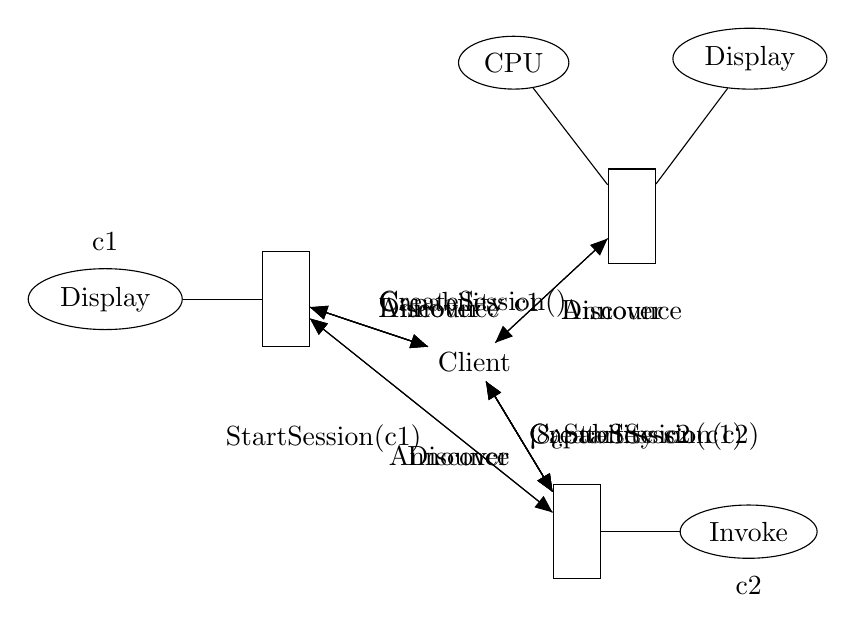
\begin{tikzpicture}[
                bidi/.style={draw, triangle 45-triangle 45},
                invoke/.style={draw, -triangle 45},
                server/.style={draw, rectangle, minimum height=1.2cm, minimum width=0.6cm},
                service/.style={draw, ellipse}
            ]

            \node (client) {Client};

            \visible<2->{
                \node[server, left=1.5cm of client,  yshift=0.8cm] (s1) {};
                \node[server, above=1.0cm of client, xshift=2.0cm] (s2) {};
                \node[server, below=1.3cm of client, xshift=1.3cm] (s3) {};
            }

            % Discover
            \visible<2>{
                \path[invoke] (client) to node[above right] {Discover} (s1);
                \path[invoke] (client) to node[below right] {Discover} (s2);
                \path[invoke] (client) to node[below left] {Discover} (s3);
            }

            % Announce
            \visible<3>{
                \path[invoke] (s1) to node[above right] {Announce} (client);
                \path[invoke] (s2) to node[below right] {Announce} (client);
                \path[invoke] (s3) to node[below left] {Announce} (client);
            }

            % Services
            \visible<3->{
                \node[service, left=of s1] (display) {Display};
                \path[draw] (display) -- (s1);

                \node[service, above=of s2, xshift=-1.5cm] (cpu2) {CPU};
                \node[service, above=of s2, xshift=+1.5cm] (display2) {Display};
                \path[draw] (cpu2) -- (s2);
                \path[draw] (display2) -- (s2);

                \node[service, right=of s3] (invoke) {Invoke};
                \path[draw] (invoke) -- (s3);
            }

            % CreateSession
            \visible<4>{
                \path[invoke] (client) to node[above right] {CreateSession()} (s1);
            }
            \visible<5>{
                \path[invoke] (s1) to node[above right] {Capability c1} (client);
            }
            \visible<5-10>{
                \node[above=1mm of display] {c1};
            }

            % CreateSession
            \visible<6>{
                \path[invoke] (client) to node[right] {CreateSession(c1)} (s3);
            }
            \visible<7>{
                \path[invoke] (s3) to node[right] {Capability c2} (client);
            }
            \visible<7-8>{
                \node[below=1mm of invoke] {c2};
            }

            % StartSession
            \visible<8>{
                \path[invoke] (client) to node[right] {\only<8>{StartSession(c2)}} (s3);
            }
            \visible<9->{
                \path[bidi] (client) to node[right] {} (s3);
            }

            % StartSession
            \visible<10>{
                \path[invoke] (s3) to node[below left] {StartSession(c1)} (s1);
            }
            \visible<11->{
                \path[bidi] (s3) to node[below left] {} (s1);
            }
        \end{tikzpicture}
    \end{figure}
\end{frame}

\begin{frame}{Protocol}
\end{frame}

\end{document}
